\chapter{Dise�o de las partes mec�nicas TODO}

La mayor parte de las piezas que monta Raider han sido redise�adas para mejorar su funci�n y/o permitir el alojamiento de nuevos dispositivos. Adem�s, al haber sido dise�adas con OpenSCAD, ha sido posible parametrizarlas para facilitar modificaciones futuras. Acciones como agregar a una pieza un soporte para un sensor determinado son ahora mucho mas r�pidas.

% TODO tablas de piezas

\section{Cabeza}

Uno de los principales objetivos del proyecto, el tomar datos del entorno con una c�mara, requiere  el dise�o y montaje se un soporte m�vil en el que poder albergar la webcam. Se ha decidido colocar la webcam en la cabeza del robot por ser la zona mas alta del robot y por tener espacio para su libre movimiento.La cabeza estar� formada por cuatro piezas: Bancada del servo, ch�sis, tapa con ranura para el cable y soporte de la c�mara.

\section{Cintura}

Como se coment� en el apartado TODO , ha sido necesario incluir un servo adicional en la cintura que permita realizar movimientos horizontales del tronco del robot respecto a la piernas. Consta de dos piezas que aprisionan el servomotor y otra mas que se utilizar� como soporte de la bater�a.


\section{Tronco}

Para dise�ar el tronco exiten varias premisas. Necesitamos un cuerpo que permita albergar el nuevo controlador, soportar los servos de los hombros, tener una zona adecuada para montar la cabeza y una base firme que permita atornillarlo al nuevo servo de la cintura.

\section{Brazos}

En este apartado se han dise�ado diferentes tramos tramos del brazo. Con ello se ha dotarle de una total modularidad, separando uniones entre servos, soportes para sensores y protectores. Gracias a esto, es muy sencillo sustituir unas piezas por otras. En este caso se han inclu�do sensores infrarrojos en los antebrazos, sin embargo, si se necesitase cambiarlos por sensores de ultrasonidos (o cualquier otro sensor) solo ser�a necesario modificar y reimprimir la bancada del sensor.

\section{Piernas}

En cuanto a las piernas, se han modificado con dos objetivos: Rigidificar sus tramos y acortar levemente su longitud para descargar peso en las articulaciones.

\section{Pies y tobillos}

El dise�o de los pies se ha planteado de forma que cumpla las especificaciones del reglamento del campeonato CEABOT y al mismo tiempo tenga la mayor superficie posible. A priori, parece sencillo suponer que cuanto mayor sea la extensi�n del pie mayor ser� la estabilidad del robot, sin embargo, tambi�n es muy importante controlar como se distribuye el peso en la planta. Con el objetivo de centrar el peso en el centro del pie, se ha realizado un redise�o completo del tobillo.

\section{Lista de piezas}

\begin{table}[h]
\centering
\begin{tabular}{ >{\centering\arraybackslash}m{4cm} >{\arraybackslash}m{2cm}  >{\centering\arraybackslash}m{1cm}  >{\centering\arraybackslash}m{4cm}}
\hline
Imagen & Archivo & Cantidad & Observaciones  \\
\hline \hline
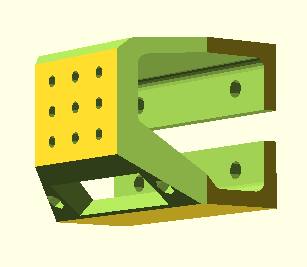
\includegraphics[width=40mm]{figuras/antebrazo} & antebrazo.stl & x1 &  \\ \hline
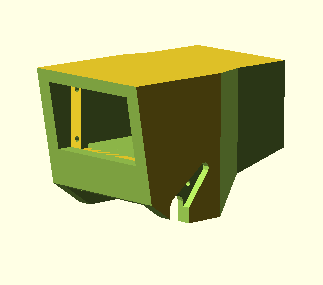
\includegraphics[width=40mm]{figuras/cabeza} & cabeza.stl & x1 &  \\ \hline
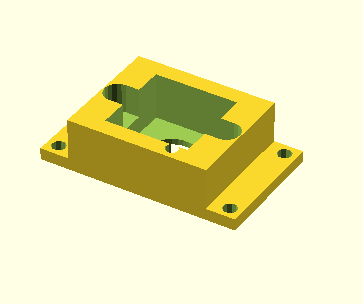
\includegraphics[width=40mm]{figuras/chasislifecam} & chasislifecam.stl & x1 &  \\ \hline
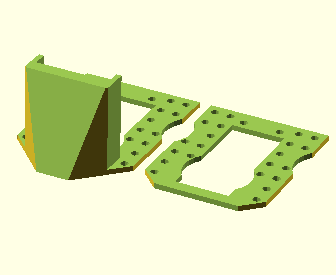
\includegraphics[width=40mm]{figuras/cintura} & cintura.stl & x1 &  \\ \hline
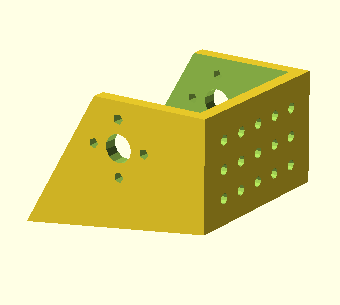
\includegraphics[width=40mm]{figuras/codo} & codo.stl & x1 &  \\ \hline
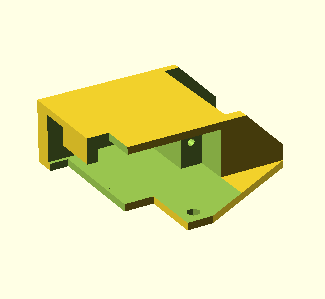
\includegraphics[width=40mm]{figuras/cuello} & cuello.stl & x1 &  \\ \hline 
\hline
\end{tabular}
\caption{piezas}
\label{tabl}
\end{table}


\begin{table}[h]
\centering
\begin{tabular}{ >{\centering\arraybackslash}m{4cm} >{\arraybackslash}m{2cm}  >{\centering\arraybackslash}m{1cm}  >{\centering\arraybackslash}m{4cm}}
\hline
Imagen & Archivo & Cantidad & Observaciones  \\
\hline \hline
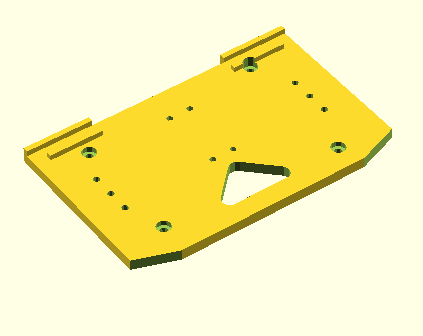
\includegraphics[width=40mm]{figuras/espalda} & espalda.stl & x1 &  \\ \hline
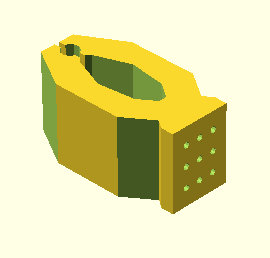
\includegraphics[width=40mm]{figuras/gripper} & gripper.stl & x1 &  \\ \hline
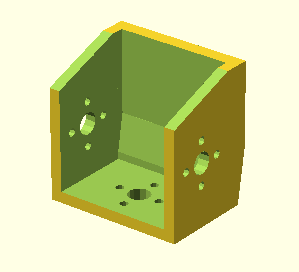
\includegraphics[width=40mm]{figuras/hombro} & hombro.stl & x1 &  \\ \hline
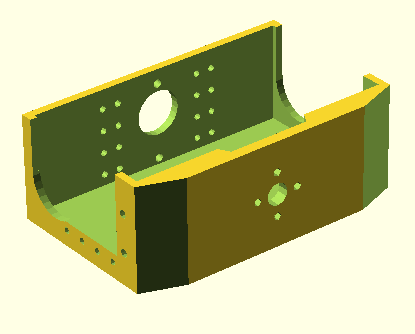
\includegraphics[width=40mm]{figuras/pecho} & pecho.stl & x1 &  \\ \hline
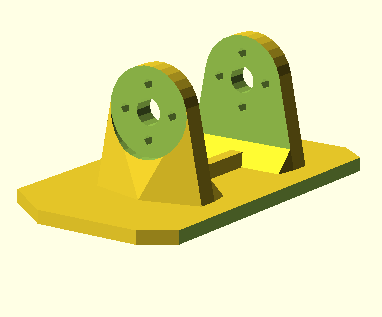
\includegraphics[width=40mm]{figuras/pie} & pie.stl & x1 &  \\ \hline
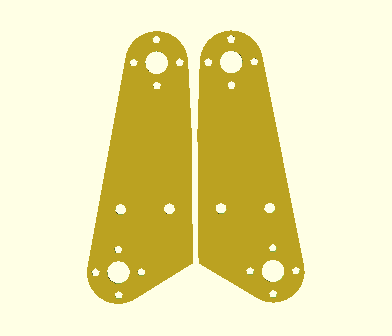
\includegraphics[width=40mm]{figuras/pierna1} & pierna1.stl & x1 &  \\ \hline
\hline
\end{tabular}
\caption{piezas}
\label{tabl}
\end{table}


\begin{table}[h]
\centering
\begin{tabular}{ >{\centering\arraybackslash}m{4cm} >{\arraybackslash}m{2cm}  >{\centering\arraybackslash}m{1cm}  >{\centering\arraybackslash}m{4cm}}
\hline
Imagen & Archivo & Cantidad & Observaciones  \\
\hline \hline
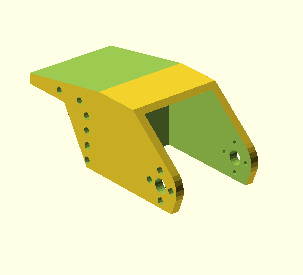
\includegraphics[width=40mm]{figuras/pierna2} & pierna2.stl & x1 &  \\ \hline
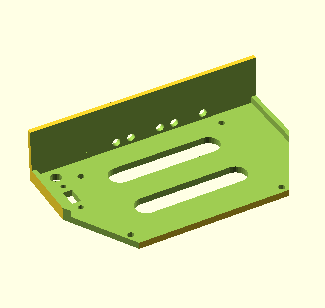
\includegraphics[width=40mm]{figuras/protector} & protector.stl & x1 &  \\ \hline
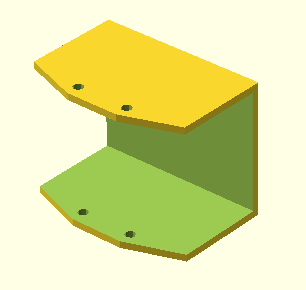
\includegraphics[width=40mm]{figuras/soportebat} & soporteBateria.stl & x1 &  \\ \hline
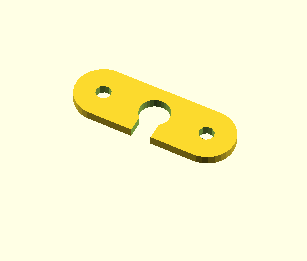
\includegraphics[width=40mm]{figuras/tapacabeza} & tapaCabeza.stl & x1 &  \\ \hline
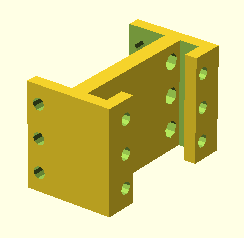
\includegraphics[width=40mm]{figuras/tobillo} & tobillo.stl & x1 &  \\ \hline
\hline
\end{tabular}
\caption{piezas}
\label{tabl}
\end{table}


